\chapter{WWW視覚化}
\label{chap:visualize}

この章では、WWW視覚化という目線での先行研究や開発事例、そして解決方法についての案を提起する。

\section{開発事例}
この分野における開発事例や先行研究は多数存在しているが、中でも3次元CGによる視覚化を実現しているUNIXソフトウェア「納豆ビュー\cite{natto}」と、mashupによる検索エンジンのWWW視覚化を実現しているWebサービス「Flowser\cite{flowser}」について解説する。

\subsection{納豆ビュー}
\begin{figure}[htbp]
\begin{center}
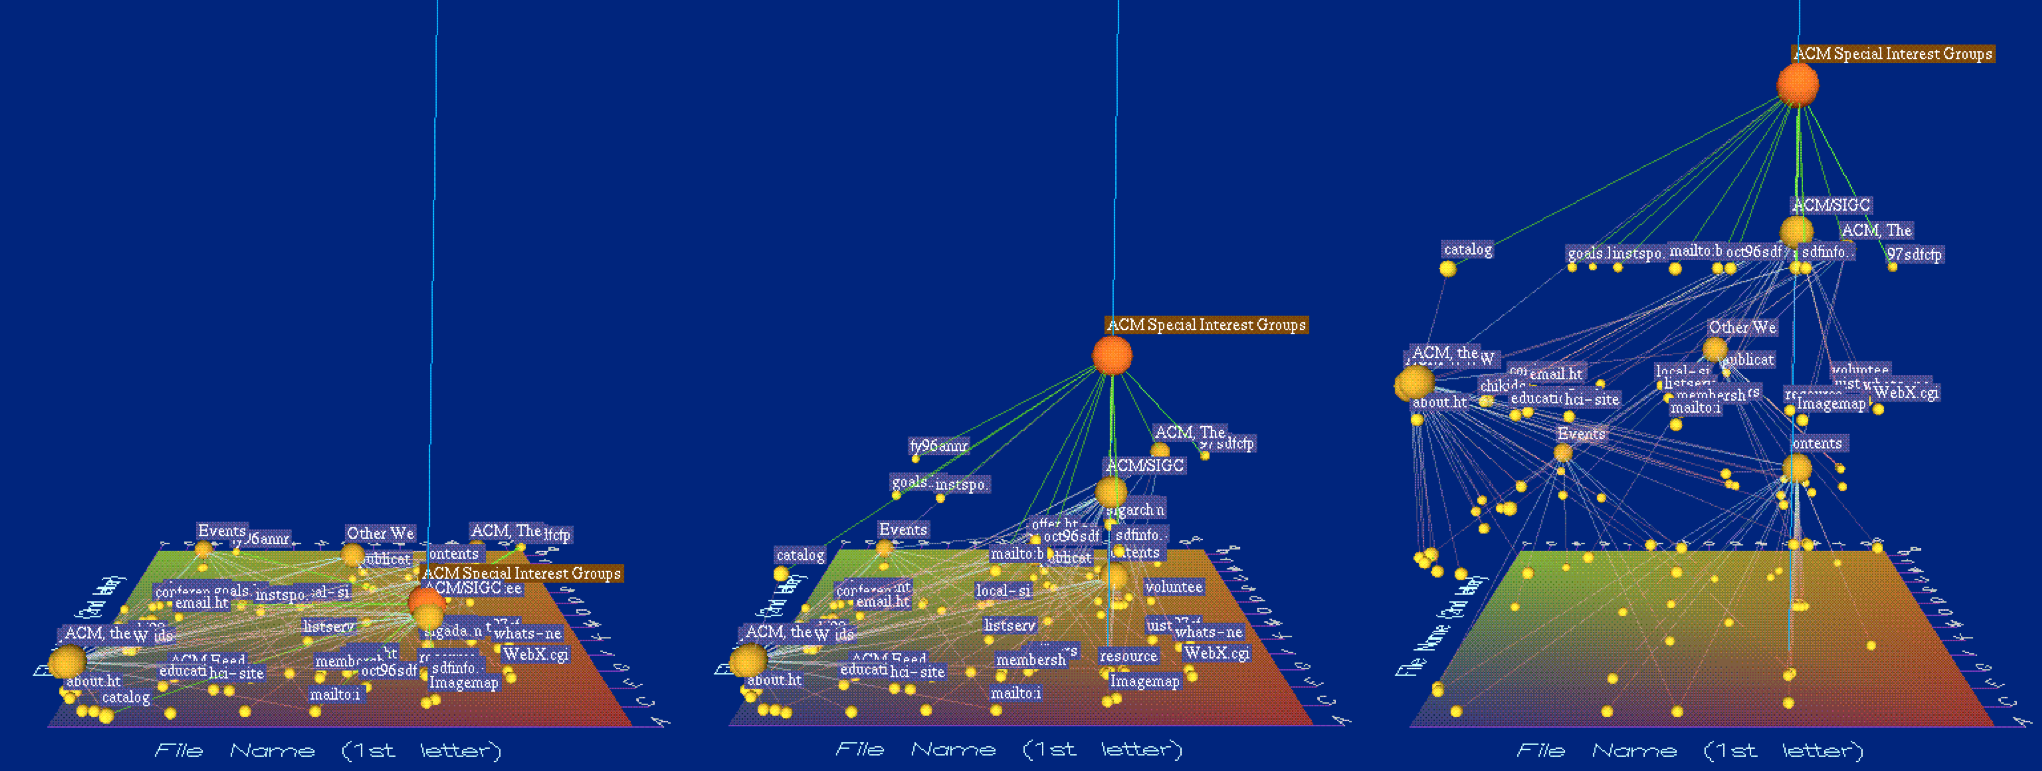
\includegraphics[width=15cm]{eps/natto.eps}
\caption{納豆ビュー}
\label{納豆ビュー}
\end{center}
\end{figure}
UNIXのX-Window System、Mesa、GLUTを用いており、3次元CGグラフ上に展開したノードをリンクに見立て、リンク・被リンクにある関係がエッジで表示される。xy平面には一意的な座標が与えられ、z軸方向にはノードを摘んで持ち上げる、つまりユーザによる操作が可能となっている。これにより、複雑なネットワークをユーザーの意志によってわかりやすく可視化できるようになっている。

\subsection{Flowser}
\begin{figure}[htbp]
\begin{center}
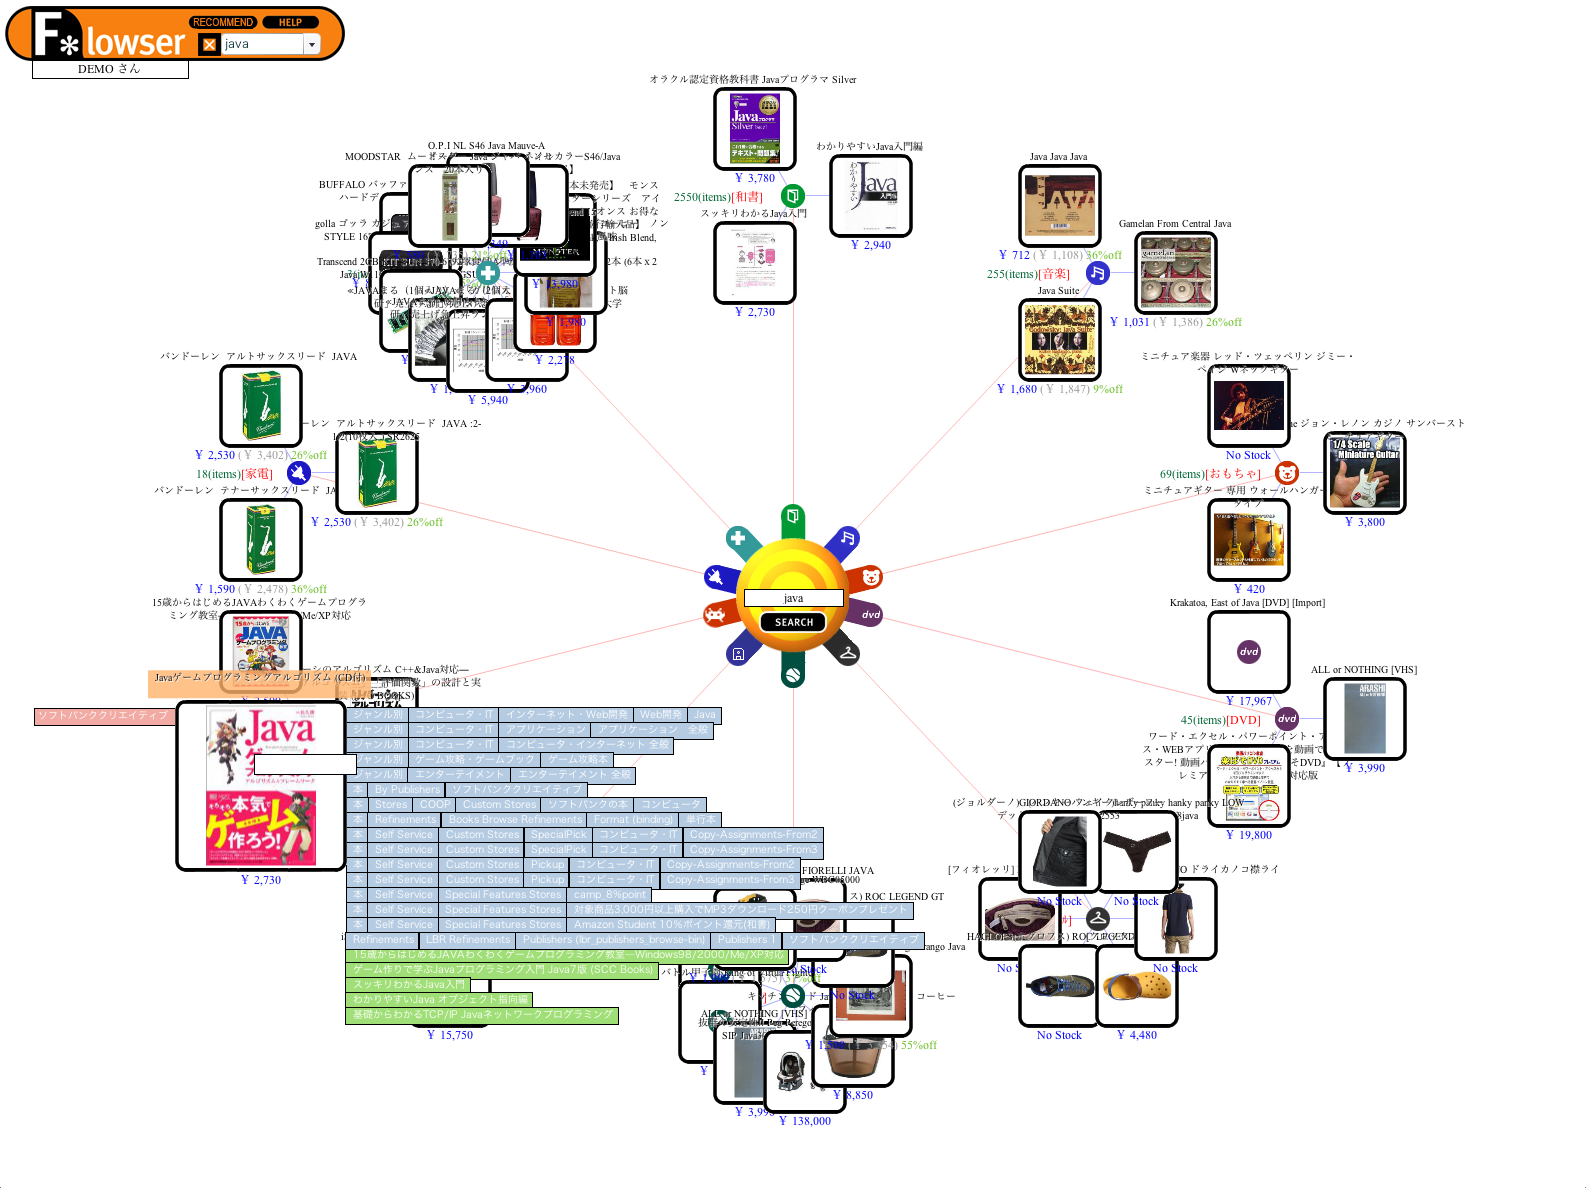
\includegraphics[width=15cm]{eps/flowser.eps}
\caption{Flowser}
\label{flowser}
\end{center}
\end{figure}
Product Advertising APIを用いたWebサービスであり、Mashupの作例でもある。検索ボックスに入力したキーワードからAmazonの複数ジャンルの商品を一気に検索・閲覧することができ、通常のサイトを通じた検索では得られなかった情報を届けることを可能にした。

\section{検索エンジンにおけるWWW視覚化}
以上2つの開発事例を見たところで、改めて、今回の研究で解決したい問題を整理する。
\begin{itemize}
\item タブレットやスマートフォン上から検索結果への直感的な操作
\\
直感的に結果を閲覧するためには、納豆ビューのようにユーザー自身によって結果をわかりやすく可視化できるようにする工夫が必要になる。また、タブレットやスマートフォンでの閲覧を前提とするため、画面サイズやボタンサイズなど、操作性に対する配慮も必要となる。
\\
\item 複数のコンテンツ(検索エンジン)を同時に検索
\\
e-learningコンテンツは、Webページだけでなく、動画、画像、PDFなどの文書ファイルのように、多数の形式に分かれていることが考えられる。であれば、Flowser.comのように、複数結果をそれぞれ分離して見やすく表示する必要がある。
\\
\item e-learningコンテンツへの導線
\\
コンテンツを検索して終了、ではなく、検索したコンテンツへはダイレクトにアクセス可能にする。ページであればブラウザでの表示を行い、動画であればタップと同時に動画サイトやアプリへ遷移し、再生を開始する必要がある。
\end{itemize}

以上の条件から、4つの表示モデルを考えた。

\subsection{Helixモデル}
\begin{figure}[htbp]
\begin{center}
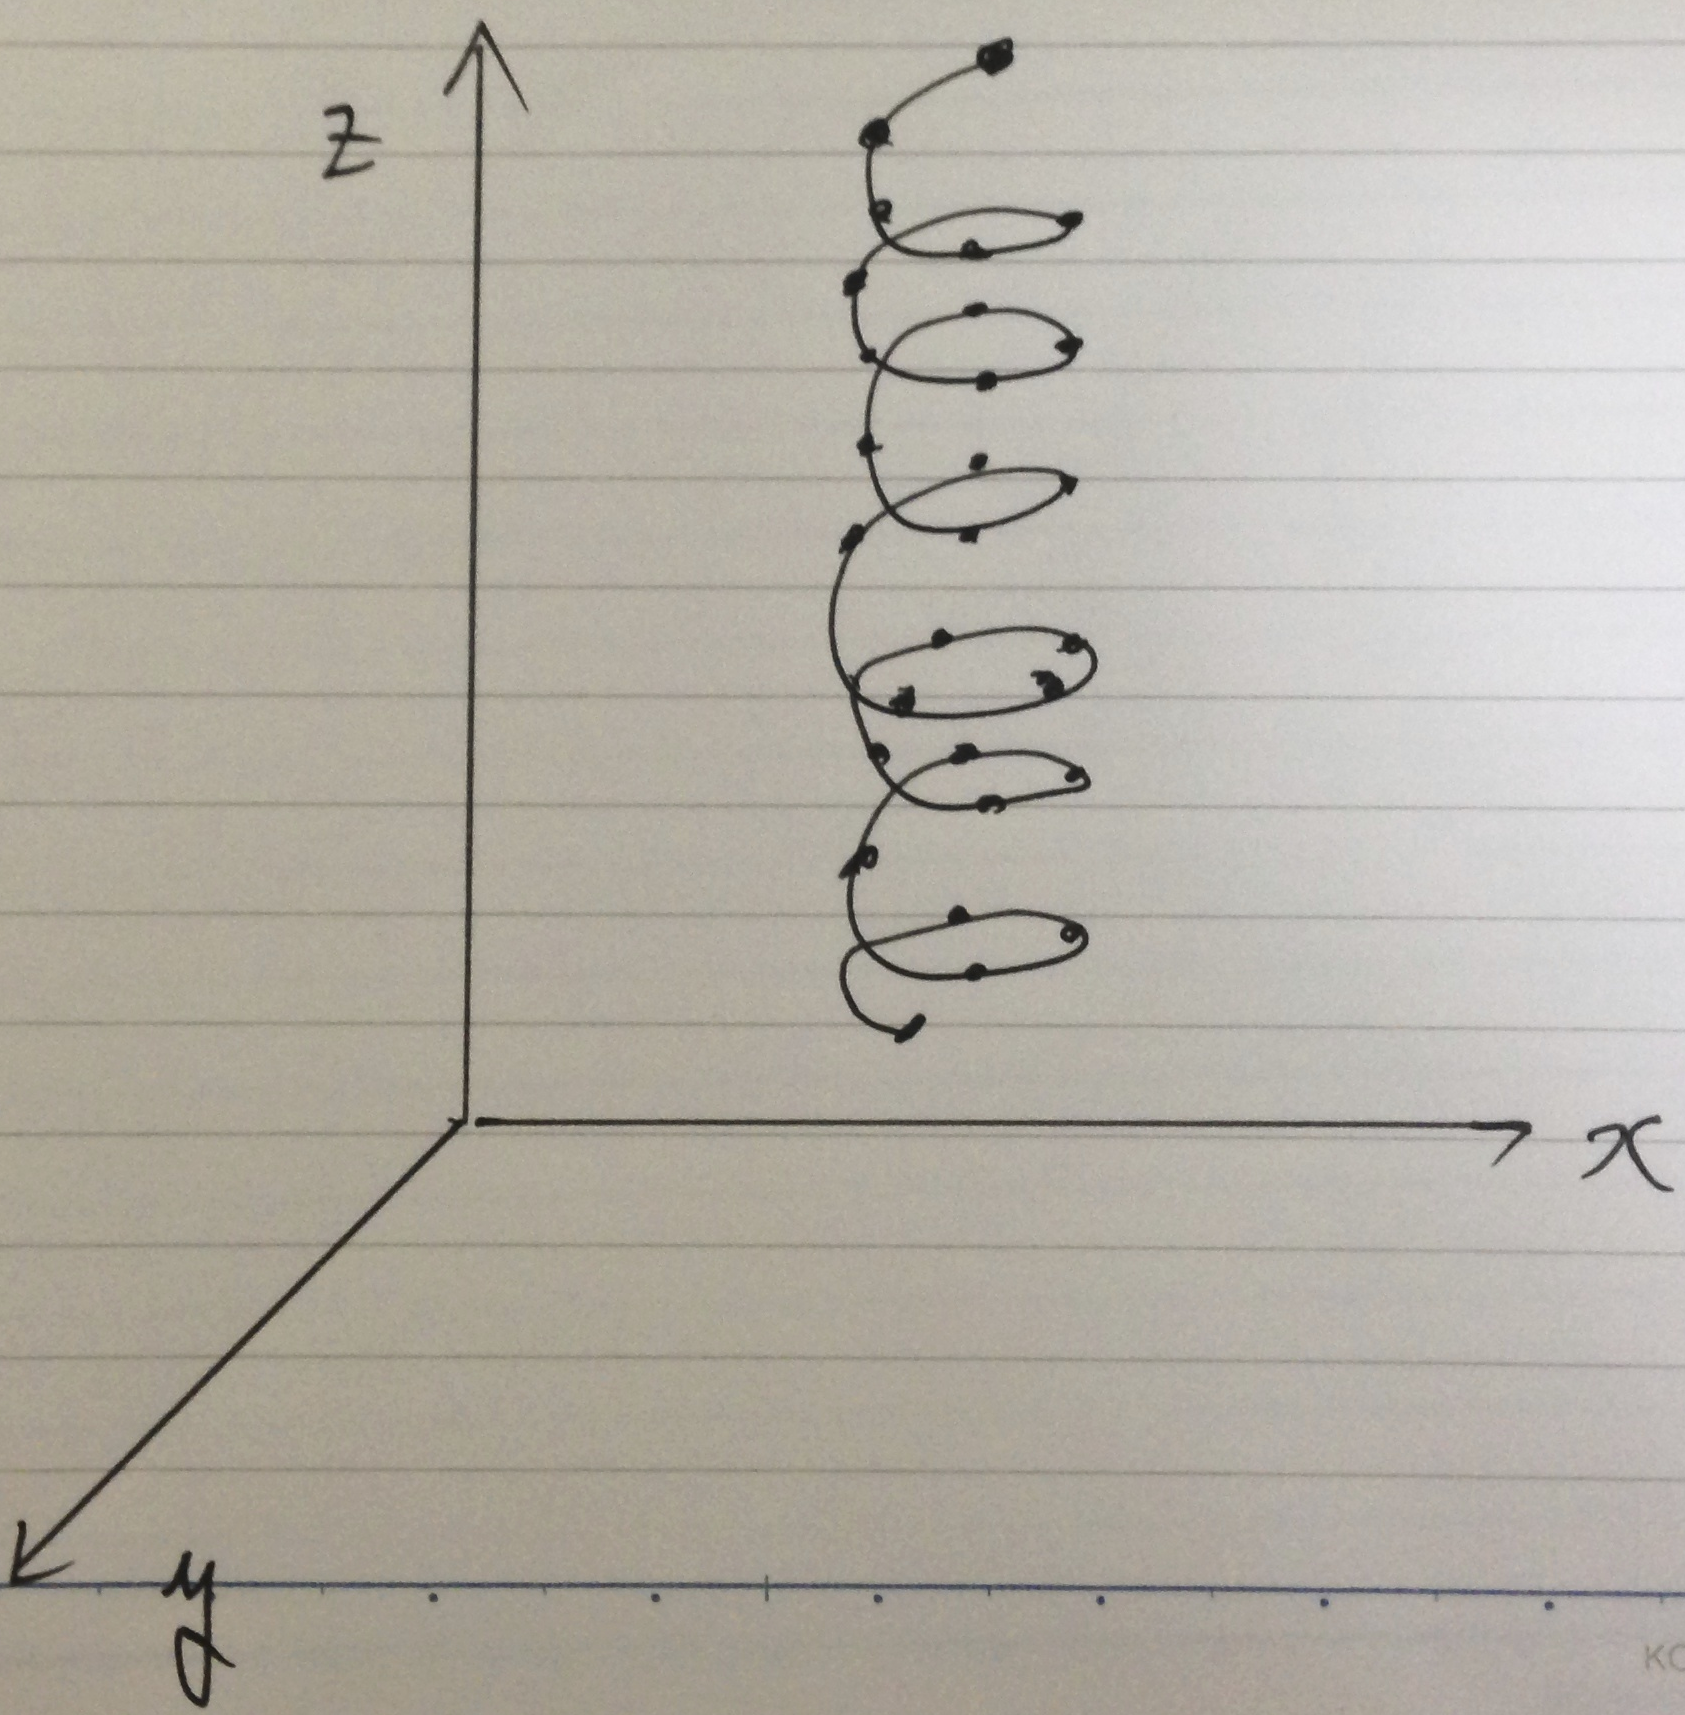
\includegraphics[width=15cm]{eps/helix.eps}
\caption{Helixモデル}
\label{helix}
\end{center}
\end{figure}
3次元螺旋の円周上に検索結果のコンテンツを配置し、螺旋階段を降りるように検索結果の下位コンテンツへと閲覧していくモデルである。この方法の優れた点として、螺旋階段の中心線からコンテンツを見た時、コンテンツ同士の下位と上位が判断しやすく、ユーザがどのような方向にスワイプしても検索結果を辿れる、つまり上下左右方向への持ち替えが容易であるといった利点がある。しかし、複数コンテンツへの対応を考えた際、螺旋一つでは画面上に対しての情報量に無駄が多く、複数コンテンツへ対応しきれない可能性が高いと考えられる。

\subsection{Starモデル}
\begin{figure}[htbp]
\begin{center}
\includegraphics[width=15cm]{eps/star.eps}
\caption{Starモデル}
\label{star}
\end{center}
\end{figure}
複数コンテンツへの配置を最優先に考え、Flowserのような円形状のコンテンツ展開を考えたモデルである。コンテンツ毎にそれぞれのノードに分類され、そこから3次元上にランダムにノードが生えており、このノードまでのエッジの長さが検索結果の上位と下位を表している。しかし、3次元上に無作為にノードが存在しているため、コンテンツの一覧性には著しく欠けており、視点を定め辛いことが考えられる。

\subsection{Star-Helixモデル}
\begin{figure}[htbp]
\begin{center}
\includegraphics[width=15cm]{eps/star-helix.eps}
\caption{Star-Helixモデル}
\label{star-helix}
\end{center}
\end{figure}
HelixモデルとStarモデル、両者のメリットをうまく併せて設計したモデルである。螺旋はコンテンツジャンルの数だけ存在し、円形状に展開した始点から同方向に対して一様に伸びている。しかし、複数の螺旋を同時に見れる視点の位置が一意に決まらないため、ユーザーが混乱する可能性が高い。

\subsection{Star-Slideモデル}
\begin{figure}[htbp]
\begin{center}
\includegraphics[width=15cm]{eps/star-line.eps}
\caption{Star-Slideモデル}
\label{star-line}
\end{center}
\end{figure}
Star modelのコンテンツ分離性を活かし、そこから垂直、同方向にコンテンツを配置したモデルである。このモデルを外周から見ると、ちょうど画面上にすべてのコンテンツが入るようになっており、非常に視認性に優れている。加えて、スワイプによって移動する方向も一意であることから、ユーザーが混乱しにくい。また、最前方に配置するコンテンツは丸型ハンガーラックのように回転するようになっており、別のコンテンツをメインに見たい、という時には横方向へのスワイプで自由に切り替えられるようになっている。

\section{採用手法}
以上より、最も多くの問題を改善できた方法として、Star-Slide モデルの採用を決定した。